\newpage

\section{Przypadki testowe} \ \ \

Zostały przygotowane 3 przykładowe przypadki testowe, które mogłyby być w zestawie testów regresyjnych dla przedstawionej aplikacji webowej.

\begin{longtable}{|l|l|
>{\columncolor[HTML]{67FD9A}}l |}
\caption{Przypadki testowe}
\label{my-label2}
\hline
\cellcolor[HTML]{EFEFEF}\textbf{Nazwa testu} & \cellcolor[HTML]{EFEFEF}\textbf{Kroki}                                                                                                                                                                                                                                                                                                                                                                                                                                                                                                                                                                                                                                                                                                                                             & \cellcolor[HTML]{EFEFEF}\textbf{Status}         \\ \hline
\endfirsthead
%
\endhead
%
TC\_LogIn\_LogOut                            & \begin{tabular}[c]{@{}l@{}}1. Otwarcie przeglądarki i przekierowanie na stronę\\ https://wordpress.com/\\ 2. Logowanie do WordPress z kontem testowym.\\ 3. Po udanym zalogowaniu się, następuje wylogowanie się.\\ 4. Zamknięcie przeglądarki.\end{tabular}                                                                                                                                                                                                                                                                                                                                                                                                                                                                                                                       & \multicolumn{1}{c|}{\cellcolor[HTML]{67FD9A}OK} \\ \hline
TC\_Add\_Comment                             & \begin{tabular}[c]{@{}l@{}}1. Otwarcie przeglądarki i przekierowanie na stronę\\ https://automationtestingwithjmeter.wordpress.com\\ 2. Napisanie komentarza pod postem.\\ 3. Przekierowanie na stronę https://wordpress.com/\\ 4. Logowanie do WordPress z kontem testowym.\\ 5. Przejście do strony Moja Witryna i wciśnięcie\\ przycisku Komentarze.\\ 4. Zatwierdzenie komentarza.\\ 5. Przekierowanie na bloga -\\ sprawdzenie, czy pojawił się komentarz na stronie.\\ 6. Powtórzenie kroków 3, 4 i 5.\\ 7. Usunięcie komentarza.\\ 8. Wylogowanie się.\\ 9. Przekierowanie na bloga -\\ sprawdzenie, czy nie ma usuniętego komentarza.\\ 10. Zamknięcie przeglądarki.\end{tabular}                                                                                          & \multicolumn{1}{c|}{\cellcolor[HTML]{67FD9A}OK} \\ \hline
TC\_Change\_Privacy                          & \begin{tabular}[c]{@{}l@{}}1. Otwarcie przeglądarki i przekierowanie na stronę\\ https://wordpress.com\\ 2. Logowanie do WordPress z kontem testowym.\\ 3. Przejście do strony Moja Witryna, a stąd do zakładki \\ Ustawienia.\\ 4. Zmiana widoczności testowanej strony na prywatną.\\ 5. Wylogowanie z platformy Wordpress.\\ 6. Przekierowanie na stronę \\ https://automationtestingwithjmeter.wordpress.com\\ 7. Sprawdzenie, czy strona zawiera komunikat, że \\ jest ona w trybie prywatnym.\\ 8. Przekierowanie na stronę https://wordpress.com.\\ 9. Powtórzenie kroków 2 oraz 3.\\ 10. Zmiana widoczności testowanej strony na publiczną.\\ 11. Powtórzenie kroków 5 oraz 6.\\ 12. Sprawdzenie, czy strona jest widoczna.\\ 13. Zamknięcie przeglądarki.\end{tabular} & {\color[HTML]{000000} OK}                       \\ \hline
\end{longtable}

\newpage

Testy zapisane w pliku CSV wyglądają następująco:

\begin{lstlisting}
===TC_LogIn_LogOut,1,
OPEN_BROWSER,dummy,
GO_TO_WEBSITE,https://wordpress.com/,
LOGIN,dummy,
LOGOUT,dummy,
CLOSE_BROWSER,dummy,
DONE
\end{lstlisting}

\begin{lstlisting}
===TC_Change_Privacy,2,
OPEN_BROWSER,dummy,
GO_TO_WEBSITE,https://wordpress.com/,
LOGIN,dummy,
ACCEPT_BUTTON,dummy,
MY_SITE_PAGE,dummy,
MODIFY_VISIBILITY,Private,
LOGOUT,dummy,
GO_TO_WEBSITE,https://automationtestingwithjmeter.wordpress.com/,
CHECK_VISIBILITY,Private,
GO_TO_WEBSITE,https://wordpress.com/,
LOGIN,dummy,
MY_SITE_PAGE,dummy,
MODIFY_VISIBILITY,Public,
LOGOUT,dummy,
GO_TO_WEBSITE,https://automationtestingwithjmeter.wordpress.com/,
CHECK_VISIBILITY,Public,
CLOSE_BROWSER,dummy,
DONE
\end{lstlisting}

\begin{lstlisting}
===TC_Add_Comment,3,
OPEN_BROWSER,dummy,
GO_TO_WEBSITE,https://automationtestingwithjmeter.wordpress.com/,
ADD_COMMENT,Czesc,
GO_TO_WEBSITE,https://wordpress.com/,
MY_SITE_PAGE,dummy,
COMMENT_OPTION,Accept,
GO_TO_WEBSITE,https://automationtestingwithjmeter.wordpress.com/,
CHECK_COMMENT,Accepted:Czesc,
GO_TO_WEBSITE,https://wordpress.com/,
MY_SITE_PAGE,dummy,
COMMENT_OPTION,Delete,
GO_TO_WEBSITE,https://automationtestingwithjmeter.wordpress.com/,
CHECK_COMMENT,Deleted:Czesc,
CLOSE_BROWSER,dummy,
DONE
END
\end{lstlisting}

Zakończenie każdego testu jest oznaczone słowem \textit{DONE}, natomiast całego zbioru testów - słowem \textit{END}. Jeżeli chcemy, żeby dany test się nie wykonał, można go zakomentować, w taki sposób, że dodajemy przed nazwą testu znak \#. Przykładowo, gdybyśmy chcieli zakomentować test TC\_Add\_Comment:
\begin{lstlisting}
#===TC_Add_Comment,3,
OPEN_BROWSER,dummy, ...
\end{lstlisting}

\begin{figure}[H]
\centering
\captionsetup{justification=centering}
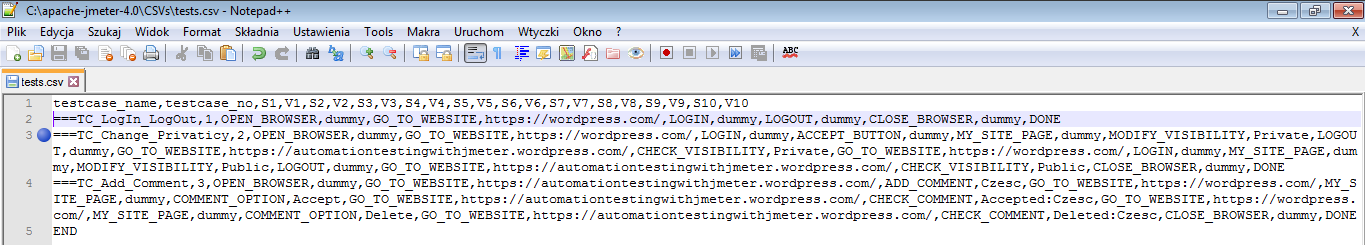
\includegraphics[width=1\textwidth]{NotePad.PNG}
\caption[Testy zapisane w pliku .csv - otwarte w programie Notepad++]{\label{fig:ham}Testy zapisane w pliku .csv - otwarte w programie Notepad++  \\ Źródło: opracowanie własne}
\end{figure}

\section{Uruchomienie testów}

Do uruchomienia testów należy otworzyć zainstalowanego wcześniej JMetera. Na rysunku 4.6 przedstawiono, jakie komendy do Wiersza poleceń na Windowsie należy wpisać, żeby otworzyć wersję graficzną JMetera, w której uruchamiamy plik \textit{Tests.jmx}. Zestaw testów został zapisany w pliku \textit{tests.csv}, do którego należy podać ścieżkę w CSV Config Element dla \textit{Tests.jmx}.

\begin{figure}[H]
\centering
\captionsetup{justification=centering}
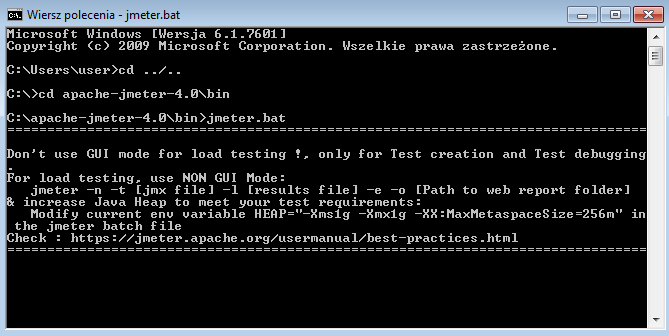
\includegraphics[width=1\textwidth]{testy_csv.png}
\caption[Sposób otworzenia JMetera - przez windowsowy wiersz poleceń]{\label{fig:ham}Sposób otworzenia JMetera - przez windowsowy wiersz poleceń \\ Źródło: opracowanie własne}
\end{figure}

\section{Wyniki wykonania testów}

Do zestawienia wyników wykonania testów w JMeterze wykorzystuje się komponent zwany \textit{Aggregate Report}, który tworzy wiersz tabeli dla każdego wykonanego kroku testowego. Zbiera informacje takie jak liczba wystąpień danego kroku, czas średni, maksymalny, minimalny wykonania czy wydajność mierzoną jako żądanie na sekundę. \cite{comp}

\begin{figure}[H]
\centering
\captionsetup{justification=centering}
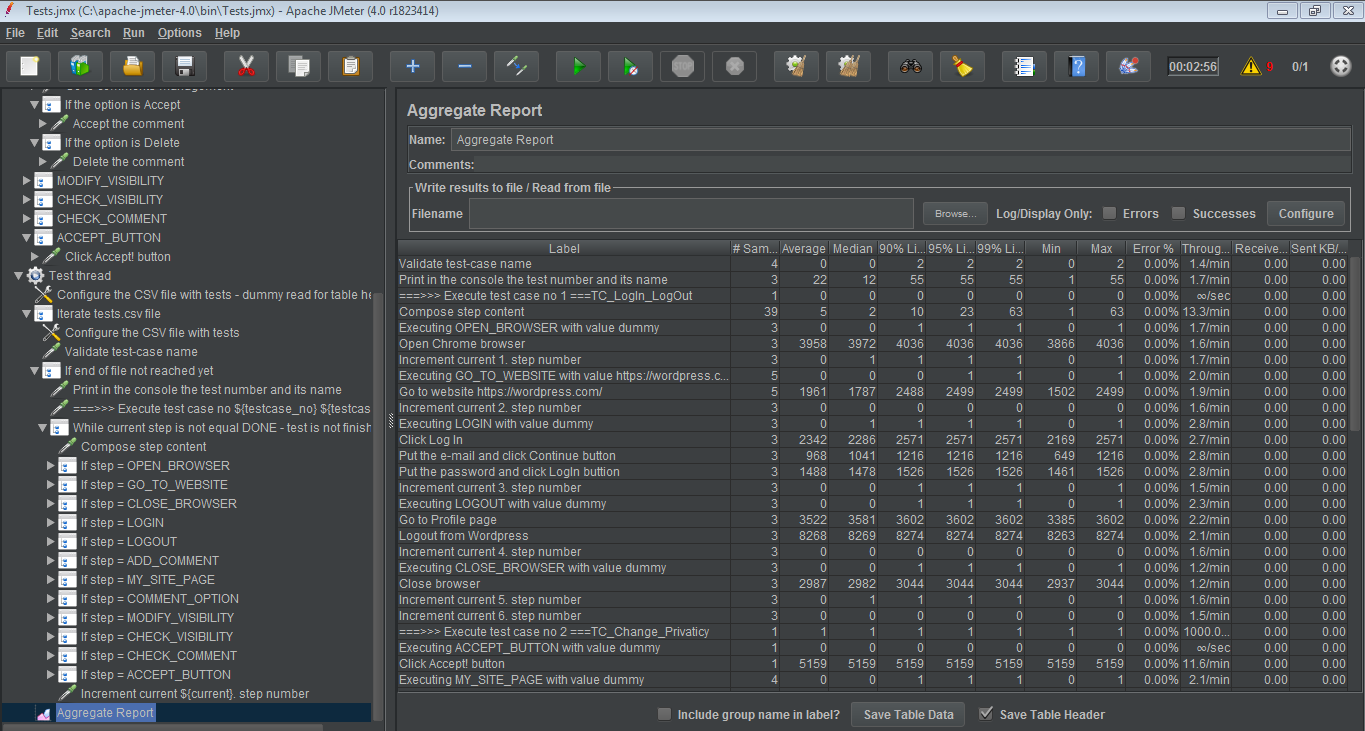
\includegraphics[width=1\textwidth]{results.PNG}
\caption[Rezultaty wykonania testów]{\label{fig:ham}Rezultaty wykonania testów \\ Źródło: opracowanie własne}
\end{figure}

Jak widać na powyższym rysunku, wykonanie trzech testów zajęło łącznie 2 minuty i 56 sekund, czyli średnio jeden test wykonał się w ciągu około 59 sekund.


Poniżej zostaną wyjaśnione parametry występujące w raporcie. Tutaj czasy są podawane w milisekundach.

\begin{itemize}
    \item \textit{Label} - Krok testowy
    \item \textit{\# Samples} - Liczba wystąpień dla tego samego kroku
    \item \textit{Average} - Średni czas wykonania zbioru rezultatów.
    \item \textit{Median} - Mediana czasu wykonania zbioru rezultatów.
    \item \textit{90\% Line} - percentyl 90\%, czyli wykonanie 90\% kroków testowych zajęło nie mniej niż podany czas.
    \item \textit{95\% Line} - percentyl 95\%, czyli wykonanie 95\% kroków testowych zajęło nie mniej niż podany czas.
    \item \textit{99\% Line} - percentyl 99\%, czyli wykonanie 99\% kroków testowych zajęło nie mniej niż podany czas.
    \item \textit{Min} - Najkrótszy czas wykonania dla kroków testowych o tej samej nazwie.
    \item \textit{Max} - Najdłuższy czas wykonania dla kroków testowych o tej samej nazwie
    \item \textit{Error \%} - Procent błędów występujących w żądaniach.
    \item \textit{Throughput} - wydajność mierzona w zapytaniach na sekundę, minutę czy godzinę.
    \item \textit{Received KB/sec} - wydajność mierzona w otrzymanych kilobajtach na sekundę.
    \item \textit{Sent KB/sec} - wydajność mierzona w wysłanych kilobajtach na sekundę.
\end{itemize}



\begin{figure}[H]
\centering
\captionsetup{justification=centering}
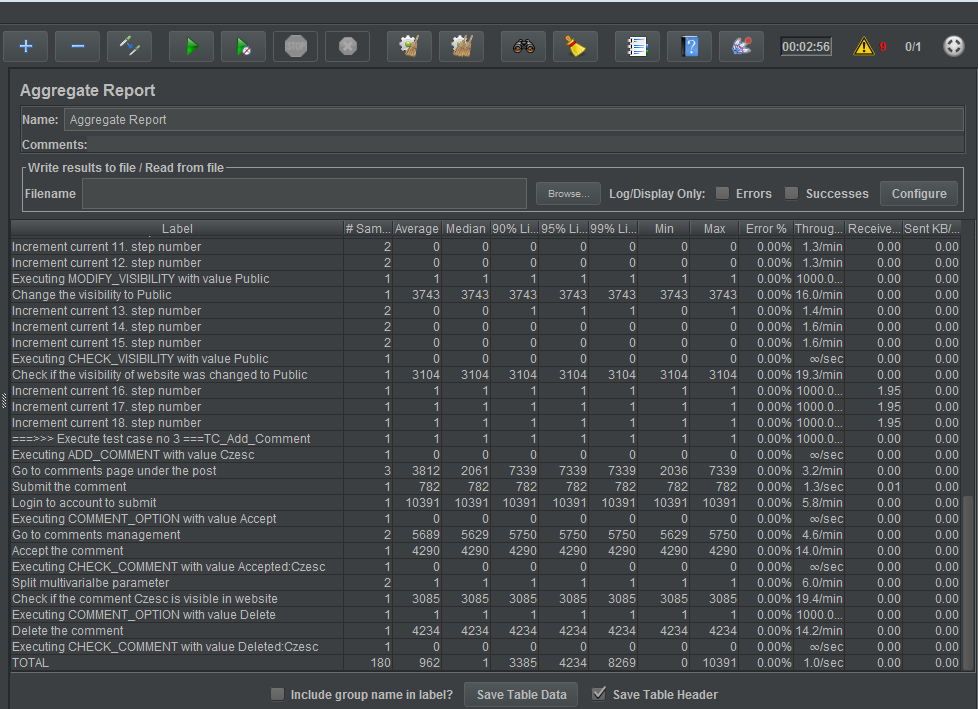
\includegraphics[width=1\textwidth]{Results2.PNG}
\caption[Rezultat wykonania testów z wierszem TOTAL podsumowującym wszystkie kroki testowe]{\label{fig:ham}Rezultat wykonania testów z wierszem TOTAL podsumowującym wszystkie kroki testowe  \\ Źródło: opracowanie własne}
\end{figure}

Analizując otrzymane wyniki dla wiersza z wartością w kolumnie Label równą TOTAL, można wyciągnąć następujące wnioski:
\begin{itemize}
    \item Wystąpiło 180 kroków testowych.
    \item Średni czas wykonania każdego z nich wynosi 962 milisekundy, czyli niecałą sekundę.
    \item Mediana jest równa 1, czyli 90 kroków testowych wykonało się co najwyżej w 1 milisekundę, a pozostałe 90 kroków powyżej 1 milisekundy.
    \item 90\% kroków testowych, czyli 162, wykonuje się w co najwyżej 3385 milisekundach. Analogicznie, 171 kroków zakończy się do 4234 milisekund, a 178 - do 8.269 sekund.
    \item Najkrótszy czas wykonania kroku testowego to 0 milisekund (czyli istnieją takie, które nic nie wykonują), natomiast najdłuższy trwał 10.391 sekund.
    \item Procent błędów dla każdego kroku testowego jest równie 0, a to oznacza, że nie wykryto żadnych błędów podczas wykonania się testów.
    \item Średnia wydajność wynosi jedno zapytanie na sekundę. Warto też zauważyć, że dla większości kroków testowych wydajność jest mierzona jako zapytanie na minutę, a dla niektórych jest ona równa $\inf$ na sekundę.
    \item Wydajność zarówno dla otrzymanych, jak i wysłanych kilobajtach na sekundach jest równa 0.
\end{itemize}


Wyniki otrzymane w Aggregate Report można zapisać w formie pliku .csv, klikając w przycisk \textit{Save Table Data}, który jest widoczny na samym dole na rysunkach 4.7. oraz 4.8.


\section{Wnioski}
Wykorzystanie rozwiązania omówionego w tym rozdziale niesie za sobą wiele korzyści. Jednym z nich jest wsparcie przez JMetera integracji z Selenium WebDriver, dzięki czemu można przeprowadzić automatyzację zarówno testów GUI, jak i aplikacji webowych. Oba narzędzia, jako że są zaimplementowane w Javie, pozwalają na napisanie testów end-to-end, wystawienie środowiska oraz przywrócenie stanu testów do początkowego.


JMeter jako narzędzie zbudowane w dużej mierze na wtyczkach może być rozszerzalne o dodatkowe wtyczki, co przykłada się na dokładniejsze sprawdzenie systemu. Można w nim też wykonać testy wydajnościowe dla istniejących scenariuszy, dodając tylko w Thread Group zwiększoną liczbę wątków.



